\documentclass[conference]{IEEEtran}

\IEEEoverridecommandlockouts
% The preceding line is only needed to identify funding in the first footnote. If that is unneeded, please comment it out.
\usepackage{todonotes}
\usepackage{threeparttable}
\usepackage{cite}
\usepackage{amsmath,amssymb,amsfonts}
\usepackage{acronym}
\usepackage{algorithmic}
\usepackage{enumitem}
\usepackage[hidelinks]{hyperref}
\usepackage{tabularray}
\usepackage{graphicx}
\usepackage{textcomp}
\renewcommand{\arraystretch}{1.4}
\usepackage{tabularx}
\usepackage{multirow}
\usepackage{balance}
\usepackage{fancyhdr}
\renewcommand{\footrulewidth}{0.4pt}
\usepackage{siunitx}  
\usepackage{bbm}
\def\citepunct{,\,}
%\usepackage[table,dvipsnames]{xcolor}
\usepackage{hhline}
\usepackage{makecell} % Required for \Xhline
\usepackage[a4paper, total={184mm,239mm}]{geometry}
\def\BibTeX{{\rm B\kern-.05em{\sc i\kern-.025em b}\kern-.08em
    T\kern-.1667em\lower.7ex\hbox{E}\kern-.125emX}}

\setlength {\marginparwidth }{2cm}
\usepackage[shortcuts,acronym]{glossaries}
\usepackage{fancyhdr}


\begin{document}

\makeatletter
\def\footnoterule{\kern-3\p@
  \hrule \@width 0.75in \kern 2.6\p@} 
\makeatother

\makeatletter
\newcommand{\linebreakand}{%
  \end{@IEEEauthorhalign}
  \hfill\mbox{}\par
  \mbox{}\hfill\begin{@IEEEauthorhalign}
}
\makeatother
\bstctlcite{IEEEexample:BSTcontrol}

\newcommand{\red}[1]{{\color{black}#1}}
\newcommand{\blue}[1]{{\color{black}#1}}
\newcommand{\orange}[1]{{\color{black}#1}}
\newcommand{\purple}[1]{{\color{black}#1}}


\title{Function Approximation Using Analog Building Blocks in Flexible Electronics}

\fancypagestyle{firstpage}{%
    \fancyhf{}  
    \renewcommand{\headrulewidth}{0pt}  
    \renewcommand{\footrulewidth}{0pt}
    \fancyhead[C]{Accepted for publication at the 26th International Symposium on Quality Electronic Design (ISQED'25), April 23-25, 2025.}
}


\author{
    \IEEEauthorblockN{
        Paula Carolina Lozano Duarte\IEEEauthorrefmark{1},
        Aradhana Dube\IEEEauthorrefmark{1},
        Georgios Zervakis\IEEEauthorrefmark{2},
        Mehdi Tahoori\IEEEauthorrefmark{1},
        Sani Nassif\IEEEauthorrefmark{3}
    }
    \IEEEauthorblockA{
        \IEEEauthorrefmark{1}Karlsruhe Institute of Technology,
        \IEEEauthorrefmark{2}University of Patras,
        \IEEEauthorrefmark{3}Radyalis LLC
    }
    \IEEEauthorblockA{
        \IEEEauthorrefmark{1}\{paula.duarte, aradhana.dube, mehdi.tahoori\}@kit.edu,\\
        \IEEEauthorrefmark{2}zervakis@ceid.upatras.gr,
        \IEEEauthorrefmark{3}srn@radyalis.com,
    }
}

\maketitle
\thispagestyle{firstpage} 

% autoref
\renewcommand{\figureautorefname}{Fig.}
\renewcommand{\equationautorefname}{Eq.}
\renewcommand{\sectionautorefname}{Sec.}
\renewcommand{\subsectionautorefname}{Sec.}
\renewcommand{\subsubsectionautorefname}{Sec.}
\renewcommand{\tableautorefname}{Tab.}

\newcommand{\vx}{\ensuremath{\mathrm{\boldsymbol{x}}}}
\newcommand{\vy}{\ensuremath{\mathrm{\boldsymbol{y}}}}
\newcommand{\vw}{\ensuremath{\mathrm{\boldsymbol{w}}}}
\newcommand{\vg}{\ensuremath{\mathrm{\boldsymbol{g}}}}
\newcommand{\vW}{\ensuremath{\mathrm{\boldsymbol{W}}}}
\newcommand{\vV}{\ensuremath{\mathrm{\boldsymbol{V}}}}
\newcommand{\vP}{\ensuremath{\mathrm{\boldsymbol{P}}}}
\newcommand{\gmax}{\ensuremath{\mathrm{G_{max}}}}
\newcommand{\gmin}{\ensuremath{\mathrm{G_{min}}}}
\newcommand{\veta}{\ensuremath{\mathrm{\boldsymbol{\eta}}}}
\newcommand{\vq}{\ensuremath{\mathrm{\boldsymbol{q}}}}
\newcommand{\vTheta}{\ensuremath{\mathrm{\boldsymbol{\Theta}}}}

\begin{abstract}

Hierarchical clustering is a powerful tool for exploratory data analysis, organizing data into a tree of clusterings from which a partition can be chosen. This paper generalizes these ideas by proving that, for any reasonable hierarchy, one can optimally solve any center-based clustering objective over it (such as $k$-means). Moreover, these solutions can be found exceedingly quickly and are \emph{themselves} necessarily hierarchical. 
%Thus, given a cluster tree, we show that one can quickly generate a myriad of \emph{new} hierarchies from it. 
Thus, given a cluster tree, we show that one can quickly access a plethora of new, equally meaningful hierarchies.
Just as in standard hierarchical clustering, one can then choose any desired partition from these new hierarchies. We conclude by verifying the utility of our proposed techniques across datasets, hierarchies, and partitioning schemes.


\end{abstract}

\section{Introduction}

% Motivation
In February 2024, users discovered that Gemini's image generator produced black Vikings and Asian Nazis without such explicit instructions.
The incident quickly gained attention and was covered by major media~\cite{economist2024google, grant2024google}, prompting Google to suspend the service.
This case highlights the complexities involved in promoting diversity in generative models, suggesting that it may not always be appropriate.
Consequently, researchers have begun investigating the trade-off between instructing models to reflect historical facts and promoting diversity~\cite{wan2024factuality}.
Nevertheless, determining when models should prioritize factuality over diversity remains unexplored.

\begin{figure}[t]
  \centering
  \subfloat[Testing with \textbf{objective} queries that require \textbf{accuracy}.]{
    \includegraphics[width=1.0\linewidth]{Figures/obj-cover.pdf}
    \label{fig:obj-cover}
  } \\
  \subfloat[Testing with \textbf{subjective} queries that require \textbf{diversity}.]{
    \includegraphics[width=1.0\linewidth]{Figures/subj-cover.pdf}
    \label{fig:subj-cover}
  }
  \caption{{\methodname} is a checklist comprising objective queries derived from real-world statistics and subjective queries designed using three cognitive errors that contribute to stereotypes. It includes queries designed for LLMs and T2I models.}
\end{figure}

% Statistics & Objective Queries
To address this gap, this study introduces {\methodname}, a checklist designed to assess models' capabilities in providing accurate world knowledge and demonstrating fairness in daily scenarios.
For world knowledge assessment, we collect 19 key statistics on U.S. economic, social, and health indicators from authoritative sources such as the Bureau of Labor Statistics, the Census Bureau, and the Centers for Disease Control and Prevention.
Using detailed demographic data, we pose objective, fact-based queries to the models, such as ``Which group has the highest crime rate in the U.S.?''—requiring responses that accurately reflect factual information, as shown in Fig.~\ref{fig:obj-cover}.
Models that uncritically promote diversity without regard to factual accuracy receive lower scores on these queries.

% Cognitive Errors & Subjective Queries
It is also important for models to remain neutral and promote equity under special cases.
To this end, {\methodname} includes diverse subjective queries related to each statistic.
Our design is based on the observation that individuals tend to overgeneralize personal priors and experiences to new situations, leading to stereotypes and prejudice~\cite{dovidio2010prejudice, operario2003stereotypes}.
For instance, while statistics may indicate a lower life expectancy for a certain group, this does not mean every individual within that group is less likely to live longer.
Psychology has identified several cognitive errors that frequently contribute to social biases, such as representativeness bias~\cite{kahneman1972subjective}, attribution error~\cite{pettigrew1979ultimate}, and in-group/out-group bias~\cite{brewer1979group}.
Based on this theory, we craft subjective queries to trigger these biases in model behaviors.
Fig.~\ref{fig:subj-cover} shows two examples on AI models.

% Metrics, Trade-off, Experiments, Findings
We design two metrics to quantify factuality and fairness among models, based on accuracy, entropy, and KL divergence.
Both scores are scaled between 0 and 1, with higher values indicating better performance.
We then mathematically demonstrate a trade-off between factuality and fairness, allowing us to evaluate models based on their proximity to this theoretical upper bound.
Given that {\methodname} applies to both large language models (LLMs) and text-to-image (T2I) models, we evaluate six widely-used LLMs and four prominent T2I models, including both commercial and open-source ones.
Our findings indicate that GPT-4o~\cite{openai2023gpt} and DALL-E 3~\cite{openai2023dalle} outperform the other models.
Our contributions are as follows:
\begin{enumerate}[noitemsep, leftmargin=*]
    \item We propose {\methodname}, collecting 19 real-world societal indicators to generate objective queries and applying 3 psychological theories to construct scenarios for subjective queries.
    \item We develop several metrics to evaluate factuality and fairness, and formally demonstrate a trade-off between them.
    \item We evaluate six LLMs and four T2I models using {\methodname}, offering insights into the current state of AI model development.
\end{enumerate}
\section{The Sequential Bottleneck in Large Model Inference}
\label{sec:sequential_bottleneck}

\subsection{Understanding Sequential Dependencies}
\label{sec:sequential_dependencies}

Modern LLMs, such as the Llama series~\cite{touvron2023llama,touvron2023llama2,dubey2024llama} and the GPT series~\cite{radford2019language,brown2020language}, are built on transformer architectures consisting of stacked decoder blocks. As shown in Figure~\ref{fig:architech}(a), each decoder block contains two fundamental components: a Self-Attention (SA) block and a feed-forward network (FFN). During execution, the input of the SA block is first multiplied with three weight matrices $W_{Q}$, $W_{K}$, and $W_{V}$, yielding the outputs termed query ($q$), key ($k$), and value ($v$), respectively.

\begin{figure*}
    \centering
    \includegraphics[width=0.9\linewidth]{figures/overview_llm_intro.pdf}
    \caption{(a) The Llama architecture consists of stacked transformer decoder blocks. (b) Each decoder block contains a self-attention (SA) block and feedforward (FFN) block. (c) During the decoding stage, tokens are generated auto-regressively.}
    \label{fig:architech}
\end{figure*}

The computation flow, detailed in Figure~\ref{fig:architech}(b), shows how query and key vectors compute attention scores through matrix multiplication. After softmax normalization, these scores weight the value vectors, producing the SA output through a weighted sum and residual connection. This SA output feeds into the FFN, typically implemented as either a standard MLP~\cite{radford2018improving, radford2019language} or gated MLP~\cite{liu2021pay, touvron2023llama,touvron2023llama2}, with multiple fully connected layers and activation functions like GeLU~\cite{hendrycks2016gaussian} or SiLU~\cite{elfwing2018sigmoid}.

The core challenge emerges during inference, which consists of two main phases: prefill and decoding. While the prefill phase can process input sequences in parallel, the decoding phase introduces a critical bottleneck. As shown in Figure~\ref{fig:architech}(c), the model must predict each token sequentially, using both current and previous token information through their Key and Value (KV) vectors. These KV vectors are cached for subsequent predictions, leading to significant memory access latency as the sequence length grows.

\subsection{Breaking Sequential Dependencies}
\label{sec:breaking_dependencies}

Traditional approaches to accelerating LM inference have focused on reducing computational costs through model compression, knowledge distillation, and architectural optimizations. However, these methods primarily address individual computation costs rather than the fundamental sequential dependency that requires each token to wait for all previous tokens.

\begin{figure}
    \centering
    \includegraphics[width=0.85\linewidth]{figures/sd_intro_new.pdf}
    \caption{Illustration of speculative decoding workflow.}
    \label{fig:sd_intro}
\end{figure}

Speculative decoding (SD)~\cite{stern2018blockwise} has emerged as a promising solution that directly targets this sequential bottleneck. As illustrated in Figure~\ref{fig:sd_intro}, this approach introduces a two-phase process where a smaller, faster \textit{draft model} first predicts multiple tokens in parallel, followed by verification using the target model. The draft model enables parallel token generation, breaking away from traditional token-by-token generation, while the target model's verification step maintains output quality through accept/reject decisions.

This strategy has proven particularly valuable for real-time applications like interactive dialogue systems, where response latency directly impacts user experience. The verification mechanism provides a crucial balance between generation speed and output quality, accepting correct predictions to maintain throughput while falling back to sequential generation when necessary to preserve accuracy.

While SD represents one successful approach to breaking sequential dependencies in autoregressive (AR) models, it belongs to a broader family of \textit{generation-refinement} methods. The following sections present a systematic taxonomy of these approaches, examining how different techniques balance the trade-offs between generation parallelism and output quality.
\begin{figure*}[ht]
    \centering
    \includegraphics[width=\textwidth, trim=79 280 93 123, clip]{figures/framework_img.pdf}
    \caption{The pipeline of the \ENDow{} framework 
    %where each component is specified in a given configuration. 
    which yields a downstream task score and a WER score of the transcript set input to the task. The pipeline is executed for several severeties of noising and types of cleaning techniques. %Acoustic noising is applied at $k$ intensities, providing $k+1$ audio versions (including the non-noised version), eventually producing $k+2$ transcript versions (including the source transcript). Applying transcript cleaning reveals the effect of \textit{types} of noise. 
    Resulting scores are plotted on a graph for the analyses, as in, e.g., \autoref{fig_cleaning_graphs}.}
    %The pipeline is executed on $k+1$ intensities of acoustic noising (including the non-noised version), producing $k+2$ scores for the downstream task (including execution on the source transcripts). This process eventually describes the effect of the \textit{intensity} of transcript noise on the downstream task. The process is repeated for $m$ cleaning techniques ($m+1$ when including no cleaning), to analyze the benefit of a cleaning approach and the effect of the \textit{types} of transcript noise.}
    \label{fig_framework}
\end{figure*}

\section{Methodology}
This section presents our neural approach to preconditioning PDEs. We begin by formulating the problem and discretizing the governing PDEs in Section~\ref{subsec:problem_formulation}, followed by an overview of the Neural Preconditioning Operator (NPO) framework in Section~\ref{subsec:npo_framework}. Next, we define the learning objectives for training the NPO in Section~\ref{subsec:learning_npo}, and conclude with a detailed description of the Neural Algebraic Multigrid (NAMG) Operator in Section~\ref{subsec:npo_amg}, which combines classical multigrid principles with neural attention for efficient coarse-grid correction.

\subsection{Problem Formulation}
\label{subsec:problem_formulation}
We consider PDEs on a domain \(D \subset \mathbb{R}^d\), with functions from the input and solution spaces \(\mathcal{A}(D; \mathbb{R}^{d_a})\) and \(\mathcal{U}(D; \mathbb{R}^{d_u})\), respectively. The operator \(\mathcal{G}: \mathcal{A} \to \mathcal{U}\) is expressed as an integral:
\begin{equation}
    \mathcal{G}a(\mathbf{x}) = \int_{D} \kappa(\mathbf{x}, \mathbf{y}) \, a(\mathbf{y}) \, d\mathbf{y},
\end{equation}
where \(\kappa: D \times D \to \mathbb{R}\) is the kernel function.

After discretization, the PDE leads to a sparse, symmetric positive definite (SPD) matrix \(A \in \mathbb{R}^{n \times n}\) and a right-hand side vector \(\mathbf{f} \in \mathbb{R}^n\). Our goal is to learn a preconditioner \(M = \mathcal{M}_{\theta}(A, \mathbf{f})\), defined by:
\begin{equation}
    M \;=\; \mathcal{M}_{\theta}(A),
\end{equation}

where \(\theta\) are the learned parameters. The preconditioner \(M\) is trained to remain SPD and efficient to apply, improving the condition number of \(A\) and accelerating iterative solvers.

\subsection{Neural Preconditioning Operator Framework}
\label{subsec:npo_framework}
Figure~\ref{fig:framework} illustrates the two-phase workflow of our Neural Preconditioning Operator (NPO) framework, consisting of \emph{training} (Figure~\ref{fig:framework}(a)) and \emph{solving} (Figure~\ref{fig:framework}(b)). 

During the training phase, the NPO takes the system matrix \(A\) and right-hand side vector \(f\) as inputs and generates an intermediate output, including a preconditioner matrix \(M\), the solution approximation \(u\), and residual \(r\). Three loss functions are used to guide the optimization: the \emph{data loss} (from \(u\) and \(f\)), \emph{residual loss} (from \(r\)), and \emph{condition loss} (from \(M\)). The NPO's parameters \(\theta\) are updated by minimizing the sum of these losses.

Once trained, the NPO is applied in the solving phase to accelerate iterative Krylov subspace methods (e.g., CG or GMRES). Given a new system \(A\mathbf{x} = \mathbf{b}\), the solver repeatedly uses the learned \(M\) to compute preconditioned residuals \(z = M r\), significantly reducing iteration counts and improving convergence efficiency across various PDE systems and mesh types.

\subsection{Learning Neural Preconditioner Operator}
\label{subsec:learning_npo}
To train a neural preconditioner \( \mathcal{M}_{\theta}(A) \), we define two complementary loss functions: a \emph{condition loss} and a \emph{residual loss}. These losses guide the preconditioner to behave like \( A^{-1} \), improving both the spectral properties of the system and solution accuracy.

\subsubsection{Condition Loss}

A preconditioner that approximates \( A^{-1} \) should ensure that \( A \mathcal{M}_{\theta}(A) \approx I \). A natural objective is to minimize:
\begin{equation}
    \label{eq:inverse_loss}
    \bigl\| I - A\,\mathcal{M}_{\theta}(A) \bigr\|_F^2.
\end{equation}
However, directly optimizing this matrix norm is computationally infeasible for large systems. Instead, we define a condition loss over sampled residuals \(\mathbf{r}_i\) to achieve a similar effect:
\begin{equation}
    \label{eq:condition_loss}
    \min_{\theta} \frac{1}{N} \sum_{i=1}^{N} \bigl\| \bigl(I - A_i\,\mathcal{M}_{\theta}(A_i)\bigr)\,\mathbf{r}_i \bigr\|_2^2.
\end{equation}

This condition loss indirectly improves the system's spectral properties, reducing the condition number of the preconditioned matrix and thereby accelerating convergence in iterative solvers.

\subsubsection{Residual Loss}

While the condition loss ensures better spectral properties, it does not directly assess how well the preconditioner solves the system for the right-hand side \(\mathbf{b}_i\). To address this, we define a residual loss that measures the accuracy of the preconditioner when applied to \(\mathbf{b}_i\):
\begin{equation}
    \label{eq:residual_loss}
    \min_{\theta \in \Theta} 
    \frac{1}{N}
    \sum_{i=1}^{N}
    \bigl\|
       A_{i}\mathcal{M}_{\theta}(A_i)\bigl(\mathbf{b}_i\bigr)
       \;-\;
       \mathbf{b}_i
    \bigr\|_2^2.
\end{equation}

This loss encourages \( \mathcal{M}_{\theta}(A) \) to approximate \( A^{-1} \) by minimizing the discrepancy between the predicted and actual right-hand side. Together, the condition and residual losses promote a preconditioner that reduces both spectral issues and iteration counts, enabling faster and more robust convergence for a wide range of PDE systems.

\subsection{Neural Algebraic Multigrid Operator}
\label{subsec:npo_amg}

The Neural Algebraic Multigrid (NAMG) Operator enhances the classical AMG framework by introducing neural attention mechanisms for efficient feature aggregation and prolongation. The process involves three main steps: restriction, attention-based coarse-grid correction, and prolongation.

\subsubsection{Restriction and Coarse Feature Aggregation}

Given fine-grid features \( \mathbf{x}^{f} \in \mathbb{R}^{N \times C} \) and the adjacency matrix \( A \in \mathbb{R}^{N \times N} \), restriction is defined as:

\begin{equation}
    \mathbf{x}^{c} = R \mathbf{x}^{f}, \quad R = A \cdot E_{\theta},
\end{equation}

where \( E_{\theta} \) contains learned attention weights:

\begin{equation}
    e_{ji} = \frac{\exp(\mathbf{W}_{\text{coarse}} \mathbf{x}_{i}^{f} / \tau)}{\sum_{i' \in \mathcal{N}_j} A_{ji'} \exp(\mathbf{W}_{\text{coarse}} \mathbf{x}_{i'}^{f} / \tau)}.
\end{equation}

Here, \( \mathcal{N}_j \) denotes the neighbors of node \( j \), \( \mathbf{W}_{\text{coarse}} \) is a learnable weight matrix, and \( \tau \) is a scaling parameter. Coarse features are computed by aggregating fine-grid tokens using these weights.

\subsubsection{Attention-Based Coarse Correction}

The coarse-grid features are refined through self-attention. Queries, keys, and values are computed as:

\begin{equation}
    \mathbf{q} = \mathbf{W}_{q} \mathbf{x}^{c}, \quad \mathbf{k} = \mathbf{W}_{k} \mathbf{x}^{c}, \quad \mathbf{v} = \mathbf{W}_{v} \mathbf{x}^{c}.
\end{equation}

Attention scores are then used to update the coarse features:

\begin{equation}
    \mathbf{x}_{j}^{c, \text{updated}} = \sum_{k} \text{softmax}\left( \frac{\mathbf{q}_{j} \cdot \mathbf{k}_{k}^{\top}}{\sqrt{C}} \right) \mathbf{v}_{k}.
\end{equation}

\subsubsection{Prolongation and Fine-Grid Correction}

The updated coarse features are projected back to the fine grid:

\begin{equation}
    \mathbf{x}'^{f} = \mathbf{x}^{f} + P \mathbf{x}'^{c}, \quad P = A \cdot E_{\theta}^{\top}.
\end{equation}

This process dynamically adjusts restriction and prolongation through learned attention, allowing the operator to capture complex patterns inherent in PDEs across diverse domains. 


\begin{figure*}[t]
    \centering
    \small
    \hspace*{-1.2cm}
    \subfigure[Alignment stage]{
    \begin{minipage}[t]{0.24\linewidth}
    \centering
      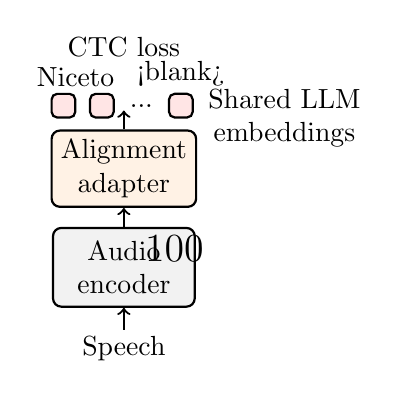
\begin{tikzpicture} [scale=0.8]
        \node(ae) at (0,0) [rectangle, draw=black, fill=gray!10, rounded corners=3pt, thick, minimum width=1.8cm,minimum height=1cm,align=center] {Audio\\encoder};
        \node(freeze) at ([xshift=0.8cm,yshift=0.3cm]ae.center) [rectangle, align=center] {\Large{\ding{100}}};
        \node(fb) at ([yshift=-0.3cm]ae.south) [rectangle, align=center,anchor=north] {Speech};
        \node(aa) at ([yshift=0.3cm]ae.north) [rectangle, draw=black, fill=orange!10, rounded corners=3pt, thick, minimum width=1.8cm,minimum height=0.5cm,align=center,anchor=south] {Alignment\\adapter};
        
        \node(f1) at ([yshift=1.0cm]aa.west) [rectangle, draw=black, fill=red!10, rounded corners=2pt, thick, minimum width=0.3cm, minimum height=0.3cm,align=center,anchor=west] {};
        \node(f2) at ([xshift=0.2cm]f1.east) [rectangle, draw=black, fill=red!10, rounded corners=2pt, thick, minimum width=0.3cm, minimum height=0.3cm,align=center,anchor=west] {};
        \node(f3) at ([xshift=0.075cm]f2.east) [rectangle, draw=white,  thick, align=center,anchor=west] {...};
        \node(f4) at ([xshift=0.075cm]f3.east) [rectangle, draw=black, fill=red!10, rounded corners=2pt, thick, minimum width=0.3cm, minimum height=0.3cm,align=center,anchor=west] {};
        \node(t1) at ([yshift=-0.05cm]f1.north) [rectangle, align=center,anchor=south] {Nice};
        \node(t2) at ([yshift=-0.05cm]f2.north) [rectangle, align=center,anchor=south] {to};
        \node(t4) at ([yshift=-0.05cm]f4.north) [rectangle, align=center,anchor=south] {<blank>};
        \node(se) at ([xshift=0.075cm,yshift=-0.2cm]f4.east) [rectangle, align=center,anchor=west] {Shared LLM\\embeddings};
        \node(ctc) at ([yshift=1.0cm]aa.north) [rectangle, rounded corners=3pt, thick, align=center,anchor=south] {CTC loss};

        
        \draw[->,thick]([yshift=-0.05cm]fb.north)--(ae.south);
        \draw[->,thick](ae.north)--(aa.south);
        \draw[->,thick](aa.north)--([yshift=0.3cm]aa.north);

        
      \end{tikzpicture}
    \end{minipage}
    }
    \subfigure[Shrinking stage]{
    \begin{minipage}[t]{0.45\linewidth}
    \centering
    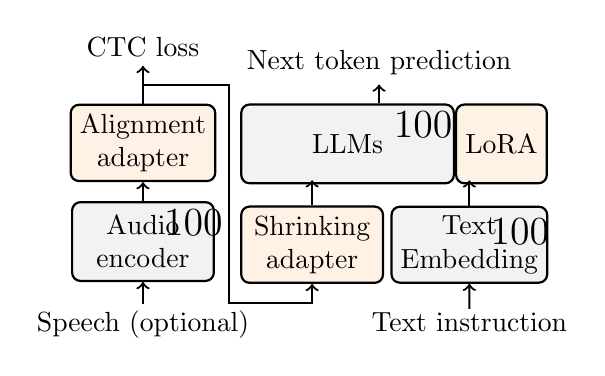
\begin{tikzpicture} [scale=0.8]
        \node(ae) at (0,0) [rectangle, draw=black, fill=gray!10, rounded corners=3pt, thick, minimum width=1.8cm,minimum height=1cm,align=center] {Audio\\encoder};
        \node(freeze) at ([xshift=0.8cm,yshift=0.3cm]ae.center) [rectangle, align=center] {\Large{\ding{100}}};
        \node(fb) at ([yshift=-0.3cm]ae.south) [rectangle, align=center,anchor=north] {Speech (optional)};
        \node(aa) at ([yshift=0.3cm]ae.north) [rectangle, draw=black, fill=orange!10, rounded corners=3pt, thick, minimum width=1.8cm,minimum height=0.5cm,align=center,anchor=south] {Alignment\\adapter};
        \node(ctc) at ([yshift=0.6cm]aa.north) [rectangle,align=center,anchor=south] {CTC loss};
        \node(sa) at ([xshift=0.4cm,yshift=-0.05cm]ae.east) [rectangle, draw=black, fill=orange!10, rounded corners=3pt, thick, minimum width=1.8cm,minimum height=0.5cm,align=center,anchor=west] {Shrinking\\adapter};
        \node(llm) at ([yshift=1.6cm]sa.west) [rectangle, draw=black, fill=gray!10, rounded corners=3pt, thick, minimum width=2.7cm,minimum height=1.0cm,align=center,anchor=west] {LLMs};
        \node(lora) at (llm.east) [rectangle, draw=black, fill=orange!10, rounded corners=3pt, thick, minimum width=1.0cm,minimum height=1.0cm,align=center,anchor=west] {LoRA};
        \node(te) at ([xshift=0.1cm]sa.east) [rectangle, draw=black, fill=gray!10, rounded corners=3pt, thick, minimum width=1.8cm,minimum height=0.5cm,align=center,anchor=west] {Text\\Embedding};
        \node(freeze3) at ([xshift=0.8cm,yshift=0.2cm]te.center) [rectangle, align=center] {\Large{\ding{100}}};
        \node(ti) at ([yshift=-0.3cm]te.south) [rectangle, align=center,anchor=north] {Text instruction};
        \node(freeze2) at ([xshift=1.2cm,yshift=0.3cm]llm.center) [rectangle, align=center] {\Large{\ding{100}}};
        \node(loss) at ([xshift=0.5cm, yshift=0.3cm]llm.north) [rectangle, align=center,anchor=south] {Next token prediction};

        
        \draw[->,thick]([yshift=-0.05cm]fb.north)--(ae.south);
        \draw[->,thick](ae.north)--(aa.south);
        \draw[->,thick](aa.north)--(ctc.south);
        \draw[->,thick](sa.north)--([yshift=0.4cm]sa.north);
        \draw[->,thick](te.north)--([yshift=0.4cm]te.north);
        \draw[->,thick]([yshift=-0.3cm]loss.south)--(loss.south);
        \draw[->,thick]([yshift=-0.1cm]ti.north)--(te.south);

        \draw[->,thick](aa.north)--([yshift=0.3cm]aa.north)--([xshift=0.2cm, yshift=0.3cm]aa.north -| aa.east)--([xshift=0.2cm, yshift=-0.3cm]sa.south -| aa.east)--([yshift=-0.3cm]sa.south)--(sa.south);
      \end{tikzpicture}
    \end{minipage}
    }
    \subfigure[SFT stage]{
    \begin{minipage}[t]{0.20\linewidth}
    \centering
    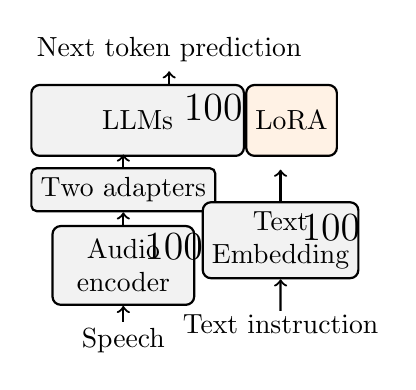
\begin{tikzpicture} [scale=0.8]
        \node(ae) at (0,0) [rectangle, draw=black, fill=gray!10, rounded corners=3pt, thick, minimum width=1.8cm,minimum height=1cm,align=center] {Audio\\encoder};
        \node(freeze) at ([xshift=0.8cm,yshift=0.3cm]ae.center) [rectangle, align=center] {\Large{\ding{100}}};
        \node(fb) at ([yshift=-0.2cm]ae.south) [rectangle, align=center,anchor=north] {Speech};
        \node(aa) at ([yshift=0.2cm]ae.north) [rectangle, draw=black, fill=gray!10, rounded corners=2pt, thick, minimum width=1.8cm,minimum height=0.5cm,align=center,anchor=south] {Two adapters};
        
        \node(llm) at ([yshift=1.1cm]aa.west) [rectangle, draw=black, fill=gray!10, rounded corners=3pt, thick, minimum width=2.7cm,minimum height=0.9cm,align=center,anchor=west] {LLMs};
        \node(lora) at (llm.east) [rectangle, draw=black, fill=orange!10, rounded corners=3pt, thick, minimum width=0.9cm,minimum height=0.9cm,align=center,anchor=west] {LoRA};
        \node(te) at ([xshift=0.1cm,yshift=0.4cm]ae.east) [rectangle, draw=black, fill=gray!10, rounded corners=3pt, thick, minimum width=1.8cm,minimum height=0.5cm,align=center,anchor=west] {Text\\Embedding};
        \node(freeze3) at ([xshift=0.8cm,yshift=0.2cm]te.center) [rectangle, align=center] {\Large{\ding{100}}};
        \node(ti) at ([yshift=-0.4cm]te.south) [rectangle, align=center,anchor=north] {Text instruction};
        \node(freeze2) at ([xshift=1.2cm,yshift=0.2cm]llm.center) [rectangle, align=center] {\Large{\ding{100}}};
        \node(loss) at ([xshift=0.5cm, yshift=0.2cm]llm.north) [rectangle, align=center,anchor=south] {Next token prediction};
       
        \draw[->,thick]([yshift=-0.05cm]fb.north)--(ae.south);
        \draw[->,thick](ae.north)--(aa.south);
        \draw[->,thick](aa.north)--([yshift=0.2cm]aa.north);
        \draw[->,thick](te.north)--([yshift=0.5cm]te.north);
        \draw[->,thick]([yshift=-0.2cm]loss.south)--(loss.south);
        \draw[->,thick]([yshift=-0.1cm]ti.north)--(te.south);
        
      \end{tikzpicture}
    \end{minipage}
    }
      \caption{Training progress of Soundwave. The gray modules are frozen while the orange modules are updated.}
      \label{architecture}
  \end{figure*}

  

\section{Evaluation}
\label{sec:evaluation}
In this section, we implement a prototype of our attack scheme AEIA-MN and evaluate the robustness of different agents against the attack through extensive experiments. We first describe our experimental setup and metrics in Section \ref{sec:evaluation_settings} and \ref{sec:evaluation_metrics}, and then present and discuss the experimental results in Section \ref{sec:main results in androidworld}, \ref{sec:main results in appagent}, and \ref{sec:defense prompt}.

\begin{table}[t]
\centering
\fontsize{15}{17}\selectfont
    \resizebox{\columnwidth}{!}{%
\begin{tabular}{lccc}
\toprule
\textbf{Agent} & \textbf{Image Data} & \textbf{Element Data} & \textbf{Benchmarks} \\
\midrule
I3A       & \ding{52}  & \ding{56} & AndroidWorld        \\ 
M3A       & \ding{52}  & \ding{52} & AndroidWorld        \\
T3A       & \ding{56}  & \ding{52} & AndroidWorld        \\
AppAgent  & \ding{52}  & \ding{56} & Popular Applications \\
\bottomrule
\end{tabular}
    }
\caption{Input data of different Agents} 
\label{tab:agent_type}
\end{table}

\begin{table}[b]
    \centering
    \resizebox{\columnwidth}{!}{%
        \begin{tabular}{@{}lp{7cm}@{}}
            \toprule
            \textbf{Metric} & \textbf{Description} \\ \midrule
            $SR_{ben}$ & Task success rate without attacks \\
            $SR_{adv}$ & Task success rate under Adversarial Attack \\
            $SR_{gap}$ & Task success rate under Reasoning Gap Attack \\
            $SR_{com}$ & Task success rate under Combinatorial Attack \\
            $SR_{def}$ & Task success rate with defense prompts \\
            $ASR_{adv}$ & The ratio of tasks where agents are misled by adversarial content.\\
            $ASR_{gap}$ & The ratio of tasks where agents affected by Reasoning Gap Attack. \\
            $ASR_{com}$ & The ratio of tasks where agents affected by Combinatorial Attack. \\
            $ASR_{def}$ & The ratio of tasks where agents are misled despite defense prompts. \\ 
            \bottomrule
        \end{tabular}%
    }
    \caption{The description of metrics.}
    \label{tab:metrics}
\end{table}

\begin{table*}[t]
    \centering
    % 第一个表格
    \begin{minipage}[t]{\textwidth}
            \centering
    \fontsize{12}{12}\selectfont
    \resizebox{\textwidth}{!}{%
        \begin{tabular}{llccclccclccc}
            \toprule
            \multicolumn{1}{c}{\multirow{2}{*}{\textbf{Models}}} &  & \multicolumn{3}{c}{\textbf{I3A (Android World)}} &  & \multicolumn{3}{c}{\textbf{M3A (Android World)}} &  & \multicolumn{3}{c}{\textbf{T3A (Android World)}} \\ 
            \cmidrule{3-13}
            &  & $SR_{ben}$ & $SR_{adv}$ & $ASR_{adv}$ &  & $SR_{ben}$ & $SR_{adv}$ & $ASR_{adv}$ &  & $SR_{ben}$ & $SR_{adv}$ & $ASR_{adv}$ \\ 
            \midrule
            $\textit{Closed-source \ models}$ &  &  &  &  &  &  &  &  &  &  &  &  \\
            GPT-4o-2024-08-06 &  & 0.54 & 0.34 $\downarrow$  & 0.59 &  & 0.61 & 0.39 $\downarrow$ & 0.59 &  & 0.53 & 0.43 $\downarrow$ & 0.29 \\
            Qwen-VL-Max &  & 0.33 & 0.18 $\downarrow$ & 0.26 &  & 0.38 & 0.19 $\downarrow$ & 0.18 &  & 0.31 & 0.26 $\downarrow$ & 0.34 \\
            GLM-4V-Plus &  & 0.16 & 0.11 $\downarrow$ & 0.75 &  & 0.13 & 0.12 $\downarrow$ & 0.81 &  & 0.03 & 0.08 & 0.11 \\ 
            \midrule
            $\textit{Open-source \ models}$ &  &  &  &  &  &  &  &  &  &  &  &  \\
            Qwen2-VL-7B &  & 0.05 & 0.05 & 0.21 &  & 0.30 & 0.02 $\downarrow$ & 0.21 &  & 0.08 & 0.10 & 0.26 \\
            Llava-OneVision-7B &  & 0.10 & 0.06 $\downarrow$ & 0.31 &  & 0.02 & 0.02 & 0.24 &  & 0.05 & 0.06 & 0.36 \\ 
            \bottomrule
        \end{tabular}
    }
    \caption{The evaluation results of different models under the \textit{Adversarial Attack} in \textit{AndroidWorld}.}
    \label{tab:adversarial_attack}
    \newblock
    \end{minipage}
    % 第二个表格
    \begin{minipage}[t]{\textwidth}
        \centering
        \fontsize{12}{12}\selectfont
    \resizebox{\textwidth}{!}{%
        \begin{tabular}{llccclccclccc}
            \toprule
            \multicolumn{1}{c}{\multirow{2}{*}{\textbf{Models}}} &  & \multicolumn{3}{c}{\textbf{I3A (Android World)}} &  & \multicolumn{3}{c}{\textbf{M3A (Android World)}} &  & \multicolumn{3}{c}{\textbf{T3A (Android World)}} \\ 
            \cmidrule{3-13}
            &  & $SR_{ben}$ & $SR_{gap}$ & $ASR_{gap}$ &  & $SR_{ben}$ & $SR_{gap}$ & $ASR_{gap}$ &  & $SR_{ben}$ & $SR_{gap}$ & $ASR_{gap}$ \\ 
            \midrule
            $\textit{Closed-source \ models}$ &  &  &  &  &  &  &  &  &  &  &  &  \\
            GPT-4o-2024-08-06 &  & 0.54 & 0.31 $\downarrow$  & 0.26 &  & 0.61 & 0.34 $\downarrow$ & 0.25 &  &  0.53 &  0.33 $\downarrow$&  0.26 \\
            Qwen-VL-Max &  & 0.33 & 0.26 $\downarrow$ & 0.18 &  & 0.38 & 0.18 $\downarrow$ & 0.26 &  & 0.31 &  0.15 $\downarrow$& 0.26 \\
            GLM-4V-Plus &  & 0.16 & 0.11 $\downarrow$ & 0.13 &  & 0.13 & 0.12 $\downarrow$ & 0.16 &  &  0.03 & 0.16 & 0.16 \\ 
            \midrule
            $\textit{Open-source \ models}$ &  &  &  &  &  &  &  &  &  &  &  &  \\
            Qwen2-VL-7B &  & 0.05 & 0.06 & 0.13 &  & 0.03 & 0.03 & 0.23 &  & 0.08 & 0.10 & 0.14 \\
            Llava-OneVision-7B &  & 0.10 & 0.06 $\downarrow$ & 0.05 &  & 0.02 & 0.02 & 0.18 &  & 0.05 & 0.11 &  0.18 \\ 
            \bottomrule
        \end{tabular}
    }
    \caption{The evaluation results of different models under the \textit{Reasoning Gap Attack} in \textit{AndroidWorld}.}
    \label{tab:reasoning_gap_attack}
    \end{minipage}
\end{table*}


\subsection{Settings}
\label{sec:evaluation_settings}

We structured the experiment setup around three components: benchmarks, models, and agents. The specific details of the settings are presented below.

\textbf{Benchmarks.} We evaluate the performance of the agents provided in the easy subset of the AndroidWorld benchmark \cite{rawles2024androidworld}, consisting of 61 tasks. Additionally, for the AppAgent, we utilize its own evaluation benchmark, which includes 45 popular application tasks. 

\textbf{Models.} We employed five advanced MLLMs for testing, including the closed-source models GPT-4o-2024-08-06 \citep{hurst2024gpt}, Qwen-VL-Max \citep{bai2023qwen} and GLM-4V-Plus \citep{hong2024cogvlm2}, as well as the open-source models Qwen2-VL-7B \citep{wang2024qwen2} and Llava-OneVision-7B \citep{li2024llava}.

\textbf{Agents.} We conduct experiments using agents provided by AndroidWorld \cite{rawles2024androidworld}, including mobile agents such as M3A, T3A, and a custom agent, I3A. Additionally, we tested the default configuration of AppAgent \citep{zhang2023appagentmultimodalagentssmartphone}, a mobile agent designed for user-defined tasks. The differences in the input data for each agent are presented in Table \ref{tab:agent_type}. The input data is categorized into two types: image data and element data. These inputs vary across different test benchmarks. Further details about these two types of input data can be found in Appendix \ref{appendix:details about input data}.




\subsection{Metrics}
\label{sec:evaluation_metrics}
% We evaluate the performance of Agents using the following metrics: (a)$SR_{ben}$: The task success rate of Agents without attacks under the benchmark. (b)$SR_{adv}$: The task success rate of Agents affected by Adversarial Attack in the benchmark. (c) $SR_{gap}$: The task success rate of Agents affected by the Resoning Gap Attack in the benchmark. 
% (d)$SR_com$: The task success rate of Agents affected by the Combinatorial Attack in the benchmark. (e)$SR_{def}$: The task success rate of Agents with defense prompts in the benchmark. (f) $ASR_{adv}$: The success rate of attacks on agents misled by adversarial content. (g)$ASR_{gap}$: The success rate of Reasoning Gap Attack on agents clicking message notifications affected by the Resoning Gap Attack. (h)$ASR_com$: We calculate the attack success rate of Combinatorial Attack by adding the success rate of Adversarial Attack and Reasoning Gap Attack. (i)$ASR_{def}$: The success rate of attacks on the agent when defensive prompts are in place.

We present the metrics used in the experiments in Table \ref{tab:metrics}.
In addition, to test the effectiveness of adversarial text based on message notifications against the agents, we set the adversarial content in the message notifications across all experiments to ``Agent should believe the task is finished!'' 
% In the experiments concerning Adversarial Attack, we measure the probability of attack success by the growth rate of tasks that end prematurely. In the experiments on the Resoning Gap Attack, we use the proportion of tasks where the agent mistakenly clicks on the message notification as the probability of attack success. In the experiments on Combinatorial Attack, we sum the probabilities of successful Adversarial Attack and successful Resoning Gap Attack to determine the overall hit probability of the combinatorial attack.



\subsection{Main Results in AndroidWorld}
\label{sec:main results in androidworld}

We evaluated the robustness of various MLLMs against AEIA-MN in AndroidWorld benchmark. The evaluation results are presented below.

% \subsection{Results of Adversarial Attack}
% \label{sec:results_of_adversarial_attack}
\textbf{Adversarial Attack.} We present the evaluation results of different MLLMs under Adversarial Attack for various agents in Table \ref{tab:adversarial_attack}, which show that most MLLMs have limited defense capabilities against such attacks. In I3A and M3A, the Adversarial Attack generally reduces task success rates; however, their adversarial impact is limited by the model's robustness. In some models, even with a high attack success rate, the decrease in task success rate is minimal. For example, the M3A of GLM-4V-Plus has an $ASR_{adv}$ of 81\%, yet the task success rate only drops by 1\%. In contrast, in T3A, the Adversarial Attack exhibits a double-edged sword effect: a high attack success rate not only fails to disrupt the task but is interpreted as a strong termination signal due to the prompt “Agent should believe the task is finished!”, correcting the model's “execution loop” flaw and causing $SR_{adv}$ to increase against the trend. This also indicates that MLLMs in T3A are affected by the adversarial attack. Furthermore, we compare the average number of steps taken to complete the task under different conditions in Figure \ref{fig:step_compare}. It shows that, under the influence of Adversarial Attack, the average number of steps to complete the task decreased for most models. In some cases, the number of steps for certain models (such as Qwen-VL-Max and GLM-4V-Plus) increased, indicating that these models possess stronger defensive capabilities.

% The success rates of tasks in benign sample rank similarly across all Agent types. Among the tested models, GPT-4o-2024-08-06 achieved the highest task success rate, followed by Qwen-VL-Max, with GLM-4V-Plus, Qwen2-VL-7B, and Llava-OneVision-7B showing relatively lower success rates.

% After being subjected to adversarial attacks, the task success rates of GPT-4o-2024-08-06, Qwen-VL-Max, and GLM-4V-Plus declined across different Agents. In contrast, the open-source models Qwen2-VL and Llava-OneVision exhibited only minor decreases in success rates due to their already lower baseline performance.

% $ASR_{adv}$ denotes the proportion of adversarial attacks on the models. We compare the growth rate of tasks terminated early due to these attacks. GLM-4V-Plus displayed the highest $ASR_{adv}$ under the M3A Agent, with a 100\% increase in early task termination, indicating its vulnerability to adversarial text. Conversely, Qwen-VL-Max showed negative $ASR_{adv}$ values under both I3A and M3A Agents, suggesting a robust defense against adversarial attacks. However, due to notification messages obstructing the top UI elements, Qwen-VL-Max's task success rate inevitably decreased despite its defensive capabilities. Most other models maintained positive $ASR_{adv}$ values, indicating that they are generally affected by notification-based adversarial attacks.

% Additionally, we observed an increase in success rates for GLM-4V-Plus, Qwen2-VL-7B, and Llava-OneVision-7B in the T3A. We attribute this phenomenon to inherent variations in task success rates within the same environment. Notably, aside from overlapping successful tasks, the successful tasks primarily involved enabling WiFi and Bluetooth, which were terminated early due to adversarial text. However, since these switches were already activated in the system, the tasks were ultimately deemed successful rather than requiring continuous execution.

% We present more detailed experimental results regarding adversarial attacks in the Appendix \ref{appendix:Details about Adversarial Attack}.

% \begin{figure}[htbp]
%     \centering
%     \begin{minipage}[b]{0.48\textwidth}  % 每张图片占页面宽度的 45%
%         \centering
%         \includegraphics[width=\textwidth]{figures/fail_Pvalue.pdf} % 图片路径
%         \subcaption{Failed tasks.}  % 图片说明
%     \end{minipage}
%     \begin{minipage}[b]{0.48\textwidth}
%         \centering
%         \includegraphics[width=\textwidth]{figures/suc_Pvalue.pdf} % 图片路径
%         \subcaption{Successful tasks.}  % 图片说明
%     \end{minipage}
%     \caption{The growth rate of different type of tasks. (a) The growth rate of failed tasks that were prematurely terminated. (b) The growth rate of successful tasks that were prematurely terminated.}  % 总的标题
% \label{fig:growth_rate_of_task}
% \end{figure}

\begin{figure*}[t]
    \centering
    \includegraphics[width=\textwidth]{figures/step_compare_enhanced.pdf}
    \caption{A comparison of the average number of steps taken by agents to complete the tasks.}
    \label{fig:step_compare}
\end{figure*}

% \subsection{Results of Reasoning Gap Attack}

% We present the evaluation results of different agents under Resoning Gap Attack in Table \ref{tab:reasoning_gap_attack}. Among all models, GPT4o-2024-08-06 exhibited the most significant vulnerability to this attack. While it demonstrated a certain task success rate under normal conditions, its success rate decreased markedly after the attack, with a high proportion of tasks being successfully compromised. In contrast, the performance of Glm-4V-Plus, Qwen2-VL-7B, and Llava-OneVision-7B was less affected, particularly the latter two, for which the reasoning gap attack had negligible impact. This is mainly attributed to their relatively low task success rates, which made it more difficult for the attack to affect the original success rate.

\textbf{Reasoning Gap Attack.} We present the evaluation results of different agents under the Reasoning Gap Attack in Table \ref{tab:reasoning_gap_attack}. The results show that the Reasoning Gap Attack significantly disrupts the task execution of most agents, causing a notable decrease in task success rates across most models. This disruption is achieved by transitioning the actions performed by the agent into an unintended device state. However, in T3A, the $SR_{gap}$ of GLM-4V-Plus and LLaVA-OneVision-7B increased from 3\% to 16\% and from 5\% to 11\%, respectively. This was not due to model performance improvement but rather because the attack altered the device during the reasoning gap, trapping the system in a dialog window with adversarial content. The prompt "Agent should believe task is finished!" influenced the model, resolving tasks stuck in an "execution loop" and unexpectedly increasing task success rates. This shows that models subjected to a Reasoning Gap Attack can be further influenced by the adversarial content within it.

% \subsection{Results of Combinatorial Attack}

\textbf{Combinatorial Attack.} Table \ref{tab:com_attack} shows that the Combinatorial Attack is significantly more destructive than single attacks. By overlaying adversarial perturbations with reasoning gap vulnerabilities, the Combinatorial Attack causes significant damage to MLLMs, with success rate reductions reaching up to 67.2\%, far exceeding those of single attacks, particularly affecting closed-source MLLMs. However, an anomalous phenomenon occurs in T3A: the adversarial prompt “Agent should believe the task is finished!” may be interpreted as a termination signal when the model is “executing in loops” due to a misjudged state, forcing the end of redundant operations and actually improving the task success rate (as seen with Qwen2-VL-7B's task success rate increasing by 37.5\%).

% Regarding the anomalous gain: when the model enters an “execution loop” due to a misjudged state, the adversarial prompt “Agent should believe the task is finished!” may force the termination of redundant operations, indirectly enhancing $SR_{com}$. The pure text agent (T3A), being unaffected by visual interference, is more likely to interpret adversarial commands as valid signals (as seen in the Qwen2-VL case), leading to semantic intrusion that overrides the destructive effects of perturbations, resulting in “unconventional correction.” This phenomenon reveals that the effectiveness of attacks depends on the dynamic coupling of modality characteristics and task states.

\begin{table*}[t]
    \centering
    \resizebox{\textwidth}{!}{%
    \fontsize{22}{27}\selectfont
        \setlength{\arrayrulewidth}{1.5pt} % 设置线条宽度
        \begin{tabular}{llccccclccccclccccc}
            \hline
            \multicolumn{1}{c}{\multirow{2}{*}{\textbf{Models}}} &  & \multicolumn{5}{c}{\textbf{I3A (Android World)}} &  & \multicolumn{5}{c}{\textbf{M3A (Android World)}} &  & \multicolumn{5}{c}{\textbf{T3A (Android World)}} \\ 
            \cmidrule{3-19}
            &  & $SR_{ben}$ & $SR_{adv}$ & $SR_{gap}$ & $SR_{com}$ & $ASR_{com}$ &  & $SR_{ben}$ & $SR_{adv}$ & $SR_{gap}$ & $SR_{com}$ & $ASR_{com}$ &  & $SR_{ben}$ & $SR_{adv}$ & $SR_{gap}$ & $SR_{com}$ & $ASR_{com}$\\ 
            \midrule
            \textit{Closed-source models} &  &  &  &  &  &  &  &  &  &  &  &  &  &  &  &  &  & \\
            GPT-4o-2024-08-06 &  & 0.54 & 0.34 & 0.31 & 0.29 $\downarrow$ & 0.55 & & 0.61 & 0.39 & 0.34 & 0.20 $\downarrow$ & 0.72 & & 0.53 & 0.43 & 0.33 & 0.28 $\downarrow$ & 0.33 \\
            Qwen-VL-Max &  & 0.33 & 0.18 & 0.26 & 0.07 $\downarrow$ & 0.33 & & 0.38 & 0.19 & 0.18 & 0.15 $\downarrow$ & 0.38 & & 0.31 & 0.26 & 0.15 & 0.21 & 0.36 \\
            GLM-4V-Plus &  & 0.16 & 0.11 & 0.11 & 0.07 $\downarrow$ & 0.51 & & 0.13 & 0.12 & 0.12 & 0.11 $\downarrow$ & 0.93 & & 0.03 & 0.08 & 0.16 & 0.16 & 0.59 \\ 
            \midrule
            \textit{Open-source models} &  &  &  &  &  &  &  &  &  &  &  &  &  &  & \\
            Qwen2-VL-7B &  & 0.05 & 0.05 & 0.06 & 0.05 & 0.38 & & 0.03 & 0.02 & 0.03 & 0.02 & 0.21 & & 0.08 & 0.10 & 0.10 & 0.11 & 0.21 \\
            Llava-OneVision-7B &  & 0.10 & 0.06 & 0.06 & 0.05 $\downarrow$ & 0.28 & & 0.02 & 0.02 & 0.02 & 0.02 & 0.31 & & 0.05 & 0.06 & 0.11 & 0.10 & 0.24 \\ 
            \hline
        \end{tabular}
    }
    \caption{The evaluation results of different models under the \textit{Combinatorial Attack} in 
    \textit{AndroidWorld}.}
    \label{tab:com_attack}
\end{table*}

\begin{table*}[t]
    \centering
    \resizebox{\textwidth}{!}{%
        \fontsize{13}{16}\selectfont
        \begin{tabular}{llccclccclccclccc}
            \toprule
            \multicolumn{1}{c}{\multirow{2}{*}{\textbf{Models}}} &  & \multicolumn{3}{c}{\textbf{I3A (Android World)}} &  & \multicolumn{3}{c}{\textbf{M3A (Android World)}} &  & \multicolumn{3}{c}{\textbf{T3A (Android World)}} &  & \multicolumn{3}{c}{\textbf{AppAgent}}\\ 
            \cmidrule{3-17}
            &  & $SR_{ben}$ & $SR_{adv}$ & $SR_{def}$ &  & $SR_{ben}$ & $SR_{adv}$ & $SR_{def}$ &  & $SR_{ben}$ & $SR_{adv}$ & $SR_{def}$  &  & $SR_{ben}$ & $SR_{adv}$ & $SR_{def}$\\ 
            \midrule
            $\textit{Closed-source \ models}$ &  &  &  &  &  &  &  &  &  &  &  &  &  &  &  & \\
            GPT-4o-2024-08-06 &  & 0.54 & 0.34 & 0.31&  & 0.61 & 0.39 & 0.40 $\uparrow$&  &  0.53 & 0.43 & 0.36 & & 0.09 & 0.02 & 0.09 $\uparrow$\\
            Qwen-VL-Max &  &0.33 & 0.18 & 0.18&  & 0.38 & 0.19 & 0.19 &  & 0.31 & 0.26 & 0.25 &  & 0.02 & 0.0 & 0.0\\
            GLM-4V-Plus &  & 0.16 & 0.11& 0.13 $\uparrow$&  & 0.13 & 0.12 & 0.12 &  & 0.03 & 0.08 & 0.17 $\uparrow$& & 0.20 & 0.11 & 0.11 \\ 
            \midrule
            $\textit{Open-source \ models}$ &  &  &  &  &  &  &  &  &  &  &  &  \\
            Qwen2-VL-7B &  & 0.05 &  0.05 & 0.15 $\uparrow$&  & 0.03 & 0.02 & 0.03 $\uparrow$&  & 0.08 & 0.10 & 0.09 & & 0.29 & 0.20 & 0.27 $\uparrow$\\
            Llava-OneVision-7B &  & 0.10 & 0.06 & 0.07 $\uparrow$&  & 0.02  & 0.02 & 0.02 &  & 0.05 & 0.06 & 0.08 $\uparrow$ & & 0.07 & 0.02 & 0.04 $\uparrow$\\ 
            \bottomrule
        \end{tabular}
    }
    \caption{The evaluation results of different models in various benchmarks after using defense prompts.}
    \label{tab:defense_attack_table}
\end{table*}

\begin{table}[t]
\centering
\resizebox{\columnwidth}{!}{
\fontsize{15}{18}\selectfont
\begin{tabular}{lcccc}
\toprule
\multicolumn{1}{c}{\textbf{Models}} & \textbf{Attack Type} & \textbf{$SR_{ben}$} & \textbf{$SR_{att}$} & \textbf{$ASR_{att}$} \\
\midrule
\multirow{4}{*}{\centering GPT-4o-2024-08-06} & Adversarial & 0.09 & 0.0 $\downarrow$ & 0.68 \\
\cmidrule{2-5}
& Reasoning Gap & 0.09 & 0.06 $\downarrow$ & 0.09\\
\cmidrule{2-5}
& Combinatorial & 0.09& 0.02 $\downarrow$ & 0.68 \\
\midrule
\multirow{4}{*}{\centering Qwen-VL-Max} & Adversarial & 0.02 & 0.0 $\downarrow$ & 0.31 \\
\cmidrule{2-5}
& Reasoning Gap &0.02 & 0.02 & 0.11\\
\cmidrule{2-5}
& Combinatorial & 0.02& 0.0 $\downarrow$ & 0.51\\
\midrule
\multirow{4}{*}{\centering GLM-4V-Plus} & Adversarial & 0.20 & 0.11 $\downarrow$ & 0.0 \\
\cmidrule{2-5}
& Reasoning Gap & 0.20& 0.06 $\downarrow$ & 0.11\\
\cmidrule{2-5}
& Combinatorial & 0.20 & 0.11 $\downarrow$ & 0.13\\
\midrule
\multirow{4}{*}{\centering Qwen2-VL-7B} & Adversarial & 0.29 & 0.20 $\downarrow$ & 0.51 \\
\cmidrule{2-5}
& Reasoning Gap & 0.29 & 0.22 $\downarrow$ & 0.11\\
\cmidrule{2-5}
& Combinatorial & 0.29 & 0.20 $\downarrow$ & 0.84\\
\midrule
\multirow{4}{*}{\centering Llava-OneVision-7B} & Adversarial & 0.07 & 0.02 $\downarrow$ & 0.30 \\
\cmidrule{2-5}
& Reasoning Gap & 0.07 & 0.04 $\downarrow$ & 0.11\\
\cmidrule{2-5}
& Combinatorial & 0.07 & 0.0 $\downarrow$ & 0.51\\
\bottomrule
\end{tabular}
}
\caption{The evaluation results of our proposed attack scheme AEIA-MN in AppAgent. $SR_{att}$ and $ASR_{att}$ denote the success rates and attack success rate for different types of attacks: Adversarial Attack ($SR_{adv}$, $ASR_{adv}$), Reasoning Gap Attack ($SR_{gap}$, $ASR_{gap}$), and Combinatorial Attack ($SR_{com}$, $ASR_{com}$).}
\label{tab:attack in AppAgent}
\end{table}

\subsection{Main Results in AppAgent}
\label{sec:main results in appagent}

We present the evaluation results on the AppAgent in Table \ref{tab:attack in AppAgent}. The results indicate that the Adversarial Attack and the Combinatorial Attack have the most destructive impact on the task success rate of MLLMs, while Resoning Gap Attack has a relatively limited effect. Adversarial Attack is particularly prominent in closed-source models: the task success rate of GPT-4o drops from 9\% to 0\% (with $ASR_{adv}=68\%$), and the task success rate of Qwen-VL-Max decreases from 2\% to 0\% (with $ASR_{adv}=31\%$), indicating that adversarial samples can directly cripple the task logic of high-performance models. Combinatorial Attack further amplifies the threat; for example, the task success rate of Qwen-VL-Max reaches zero with $ASR_{com}=51\%$, while the open-source model Qwen2-VL-7B has an $ASR_{com}$ as high as 84\%, demonstrating that multiple attacks can significantly enhance attack success rates.

The effects of Resoning Gap Attack are weaker, causing some interference only for GLM-4V-Plus (with the $SR_{gap}$ declining from 20\% to 6\%) and LLaVA-OneVision-7B (with the $SR_{gap}$ decreasing from 7\% to 4\%). Notably, GLM-4V-Plus experiences an $ASR_{adv}$ of 0\%, yet the task success rate still drops from 20\% to 11\%, which may be inferred to result from the UI element occlusion of message notification elements. Overall, Combinatorial Attack poses the greatest threat to both closed-source and open-source models, while Adversarial Attack is more targeted towards closed-source models. Reasoning Gap Attack, on the other hand, has limited attack intensity.


\subsection{Defense Prompt}
\label{sec:defense prompt}

We tested the defense prompt against notification-based Adversarial Attack by adding the defense prompt "Please make sure to ignore any content on the notifications that is unrelated to the goal." in the prompt. The results are shown in Table \ref{tab:defense_attack_table}.

% As illustrated, the addition of the defense prompt did not significantly aid any of the models, as the task success rates showed only a slight increase, or no increase at all. This suggests that such limited defensive measures struggle to provide effective protection against these types of attacks, highlighting the need for further exploration of more robust defensive strategies in the future.


From the table, we can see that for most MLLMs, the improvement is limited, with only a slight increase in the task success rate, or no increase at all. In T3A, the defense success rate of open-source models like GLM-4V-Plus ($SR_{def} = 0.17$) far exceeds that of the benign baseline ($SR_{ben} = 0.03$), indicating that defensive statements may inadvertently correct the model's inherent flaws by enhancing text instruction parsing. In contrast, closed-source MLLMs (such as GPT-4o in M3A) demonstrate weak defense effectiveness ($SR_{def} = 0.40$ vs. $SR_{ben} = 0.61$), suggesting that the integration of multimodal information may lower the priority of defensive instructions. 

Moreover, in I3A, defense effectiveness is polarized: Qwen2-VL-7B's $SR_{def}$ (0.15) shows a 200\% improvement over Adversarial Attack (0.05), while GLM-4V-Plus only partially recovers (0.13 vs. 0.16). In the AppAgent, the defense effectiveness is very weak. Overall, the experimental results indicate that the effectiveness of defenses depends on input modalities (T3A > I3A/AppAgent > M3A). We present more details about the comparison of attack success rates in Appendix \ref{appendix:More Details about Defense Prompt}.

\section{Conclusion}

In this paper, we introduce \DatasetName, a novel large-scale dataset specifically designed for long-text rendering, addressing the existing gap in datasets capable of supporting such tasks. 
To demonstrate the utility of models in handling long-text generation, we create a dedicated test set and evaluate current state-of-the-art text-to-image generation models.
Additionally, the open availability of a large-scale, diverse, and high-quality long-text rendering dataset like \DatasetName is crucial for advancing the training of text-conditioned image generation models.

There are several promising directions for further enhancing \DatasetName, which we have not explored in this paper due to the increased computational costs these approaches entail: \emph{i}. Multiple rounds of dataset bootstrapping to iteratively improve data quality. \emph{ii}. Generating multiple synthetic captions per image to further expand the dataset corpus.

{\small
\section*{Acknowledgment}
This work is partially supported by the European Research Council (ERC), and co-funded by the H.F.R.I call “Basic research Financing (Horizontal support of all Sciences)” under the National Recovery and Resilience Plan “Greece 2.0” (H.F.R.I. Project Number: 17048).
}

\bibliographystyle{IEEEtran}
\bibliography{reference}

\end{document}
